\chapter{Organisation}

\section{Méthodes de travail}

Pour ce deuxième semestre, notre équipe s’est vue diminuée de deux membres : Marie-Alice Schweitzer et Laure Dupasquier. Nous avons donc dû totalement remanier notre système de fonctionnement.
Notre groupe s'est séparé en deux parties distinctes. D’un côté Katleen Blanchet, Titouan Boulmier et Pierre Jacquot ont travaillé sur la réalisation concrète du projet décrit dans le premier rapport d’avancement. Cela consistait à la création d’un système composé d’une webcam relié à un ordinateur, permettant d’enregistrer la direction du regard de l’utilisateur et de déplacer le curseur sur l’écran en fonction de cette direction.  (Les tâches spécifiques données à chacun seront décrites par la suite).

Et de l’autre Hussain Al Othman a été chargé de réaliser des recherches sur un second système. Ce second système est directement embarqué sous forme de lunettes sur l’utilisateur. Cette partie vient compléter notre rapport, en donnant une alternative à notre prototype, mais n'est pas réalisée et reste purement théorique. Elle permet d’offrir une alternative à notre projet, si celui-ci est poursuivi par la suite.

Pour ce qui est des réunions, elles étaient conduites tous les mardi matin, afin de se répartir les tâches et aussi de connaitre l’avancement de chacun dans son travail. Le rôle de secrétaire, anciennement occupé par Laure Dupasquier a été effectué par Pierre Jacquot afin de garder une trace de chaque réunion et de planifier au mieux nos actions futures.

Katleen Blanchet et Titouan Boulmier ont continué de s’occuper de la rédaction et de la mise en page du rapport ainsi que de la mise à jour de la page Git Hub.
Les livrables réalisés au cours de ce semestre ont été réalisés en majorité par Pierre Jacquot et relus par le reste de l’équipe.

\section{Outils pour les échanges}

Concernant ce semestre les échanges ont été beaucoup plus simples à effectuer. Etant trois à travailler sur la partie principale du projet, la répartition du travail a été rapide et efficace. Le déroulement des séances se faisait le matin à notre arrivée, et nous nous adaptions au fur et à mesure de la journée au travail qu’il restait à faire.
La majorité des échanges s'est fait via e-mail.
 
En dehors du projet, pour les questions de logistique (horaires de travail, lieux), nous restions en contact par mail. 

\section{Répartition des tâches dans le temps}

Afin de visualiser au mieux les tâches à effectuer dans le temps nous avons réalisé un diagramme de Gantt (voir figure \ref{fig:GanttSemestre2}).
 
\begin{figure}[H]
  \centering
  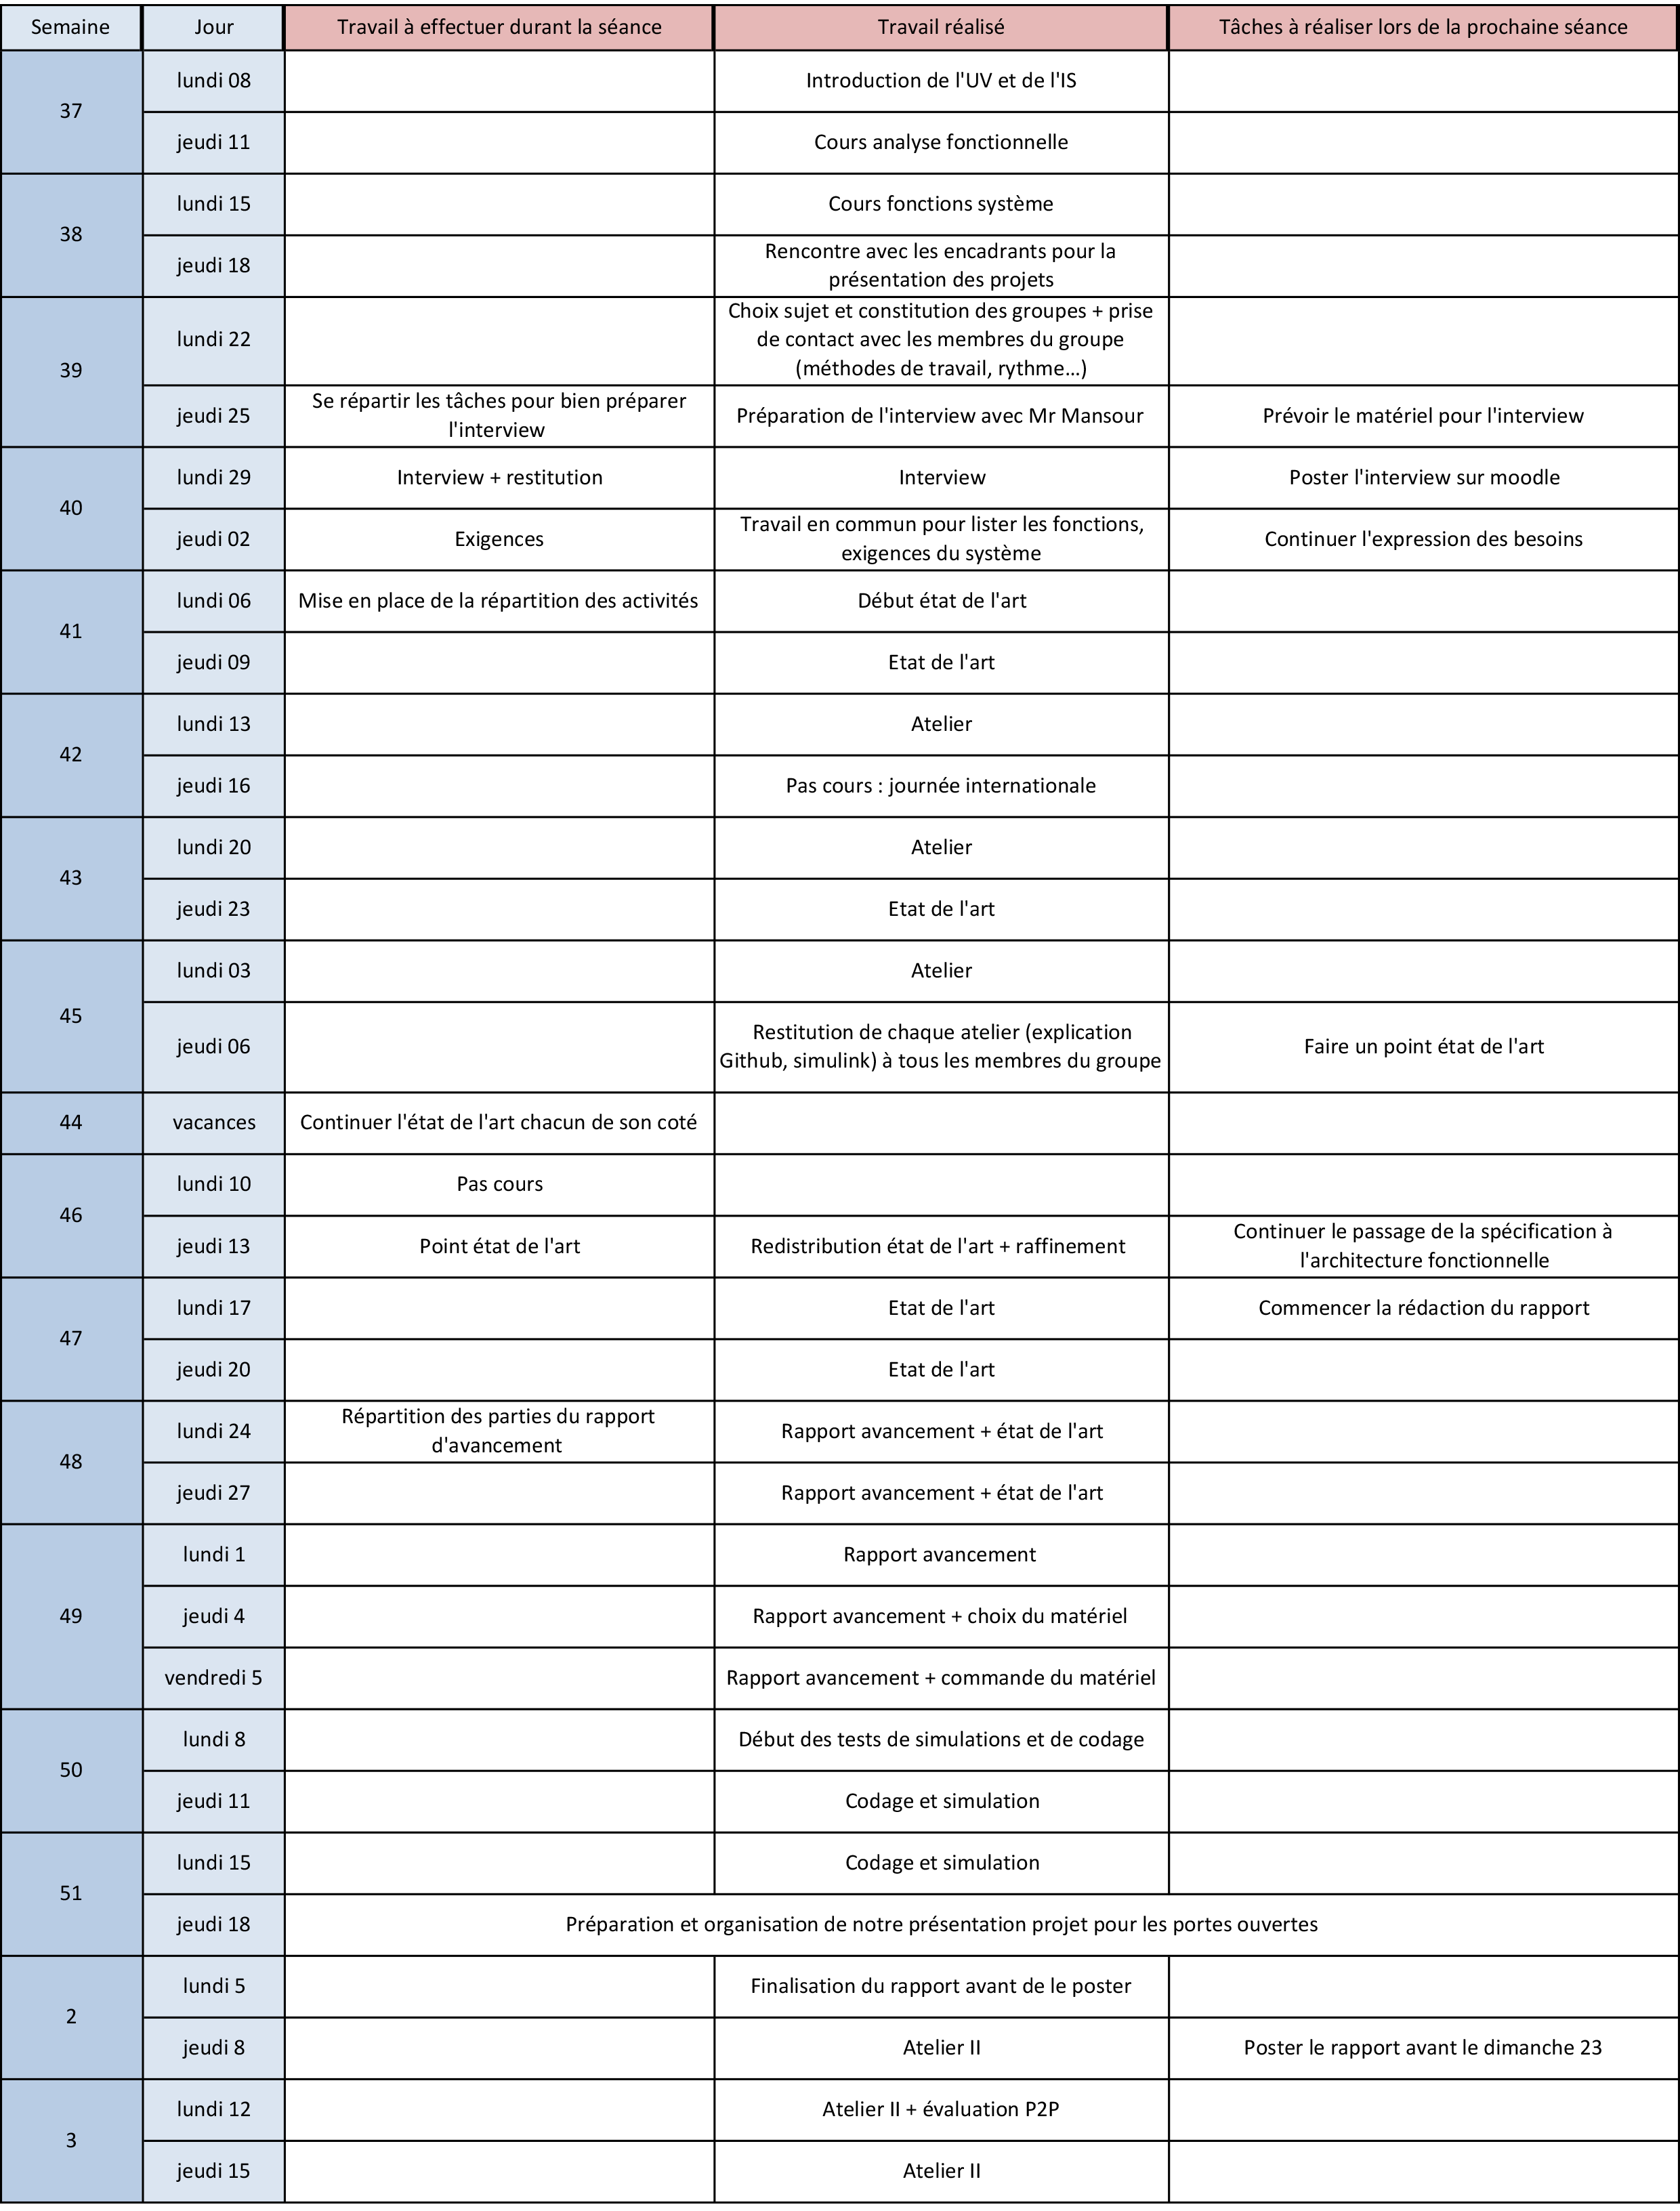
\includegraphics[scale=0.7]{CarnetBord}
  \caption{Carnet de bord semestre 1}
  \label{fig:CarnetBord}
\end{figure}

\begin{figure}[H]
  \centering
  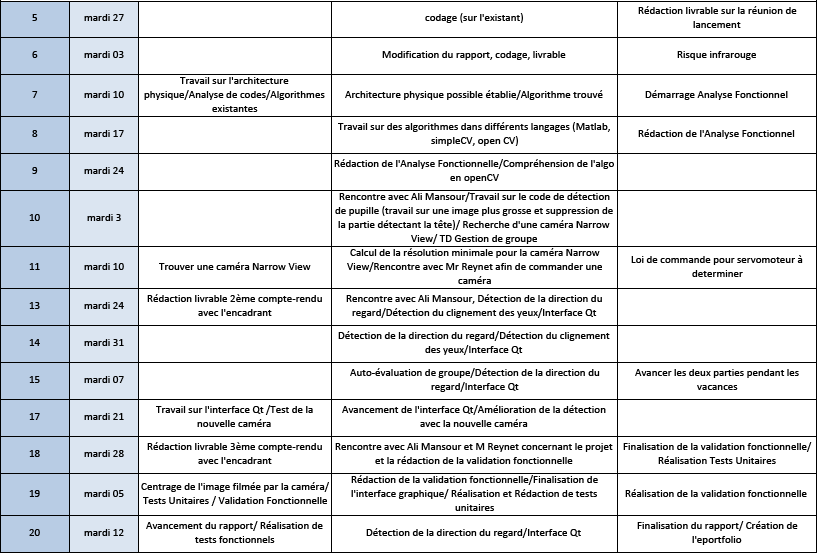
\includegraphics[scale=0.5]{CarnetBordSemestre2}
  \caption{Carnet de bord semestre 2}
  \label{fig:CarnetBordS2}
\end{figure}
 
Ce diagramme nous a permis d’anticiper au mieux les échéances, et de commencer à réfléchir aux livrables en avance. En plus de la réunion de planification, nous faisions un point sur l’avancement de chacun tous les matins.

Il est vrai que notre faible nombre a rendu l’organisation compliquée, car l’un de nous devait régulièrement interrompre ses avancées sur la partie technique, qui était pourtant cruciale car non débutée (ou peu) au premier semestre, afin de rédiger des livrables. L’équipe fonctionnait donc à 2/3 de ses possibilités sur la partie technique la plupart du temps au cours du mardi.
 
\begin{figure}[H]
  \centering
  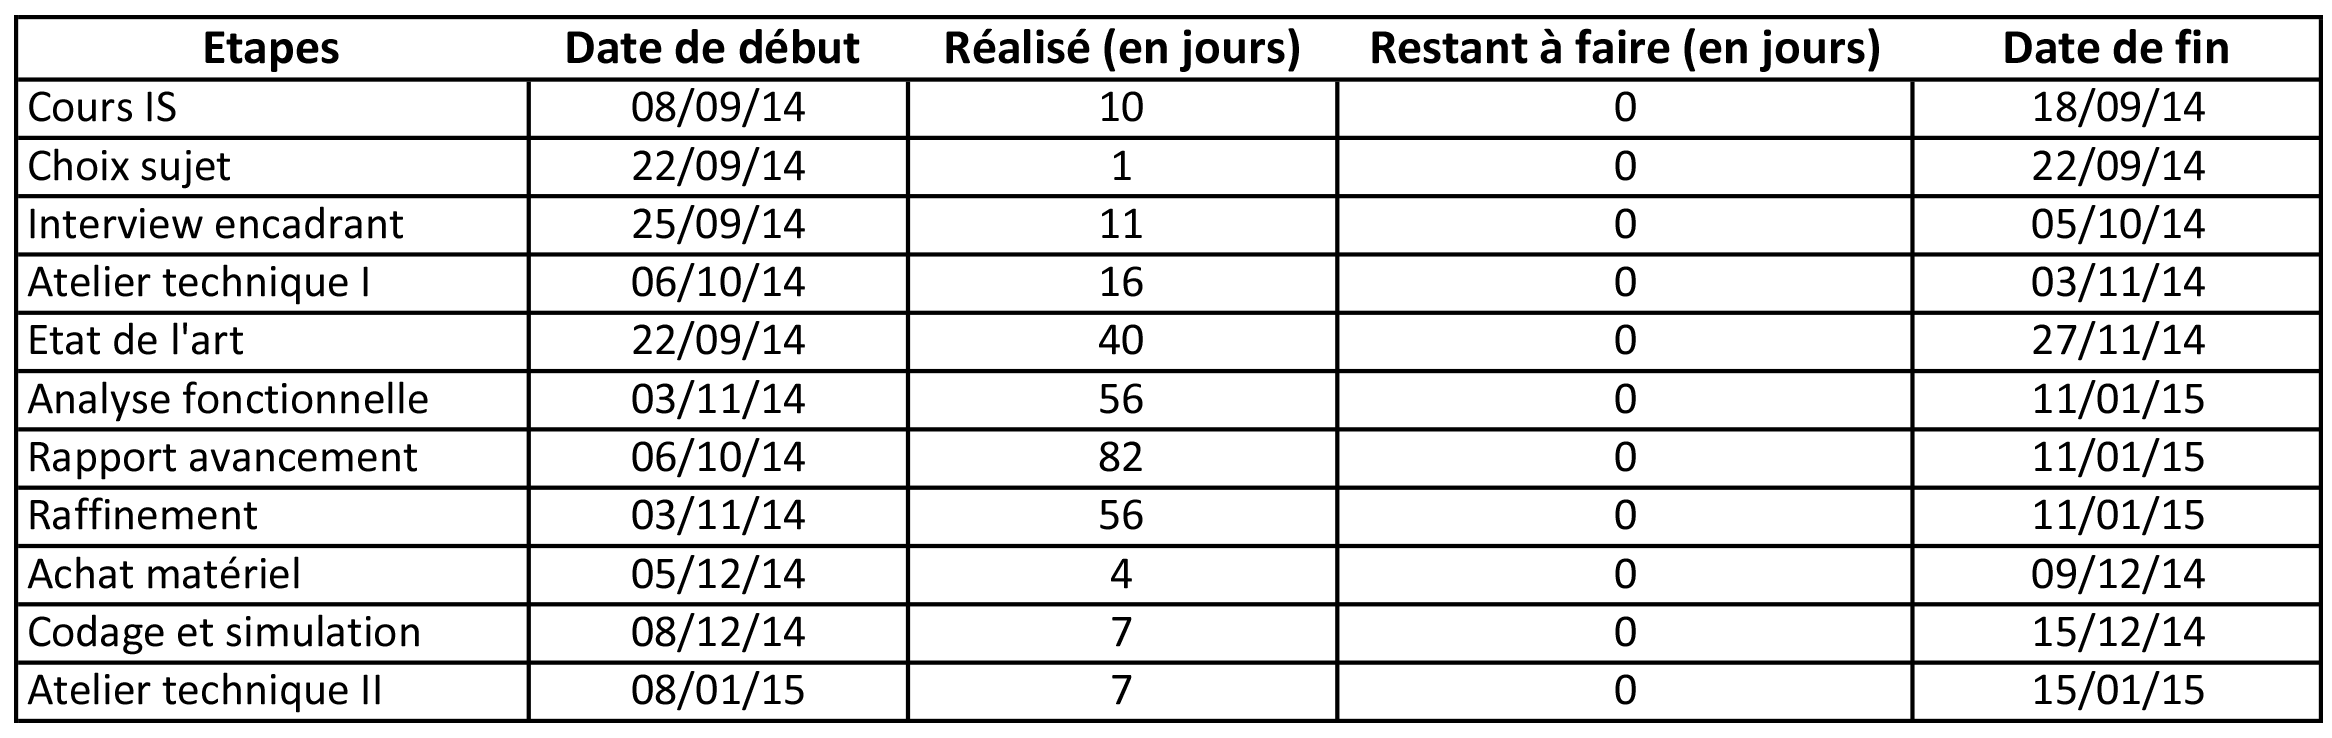
\includegraphics[scale=0.6]{Gantt}
  \caption{Diagramme de Gantt semestre 1}
  \label{fig:Gantt}
\end{figure}

\begin{figure}[H]
  \centering
  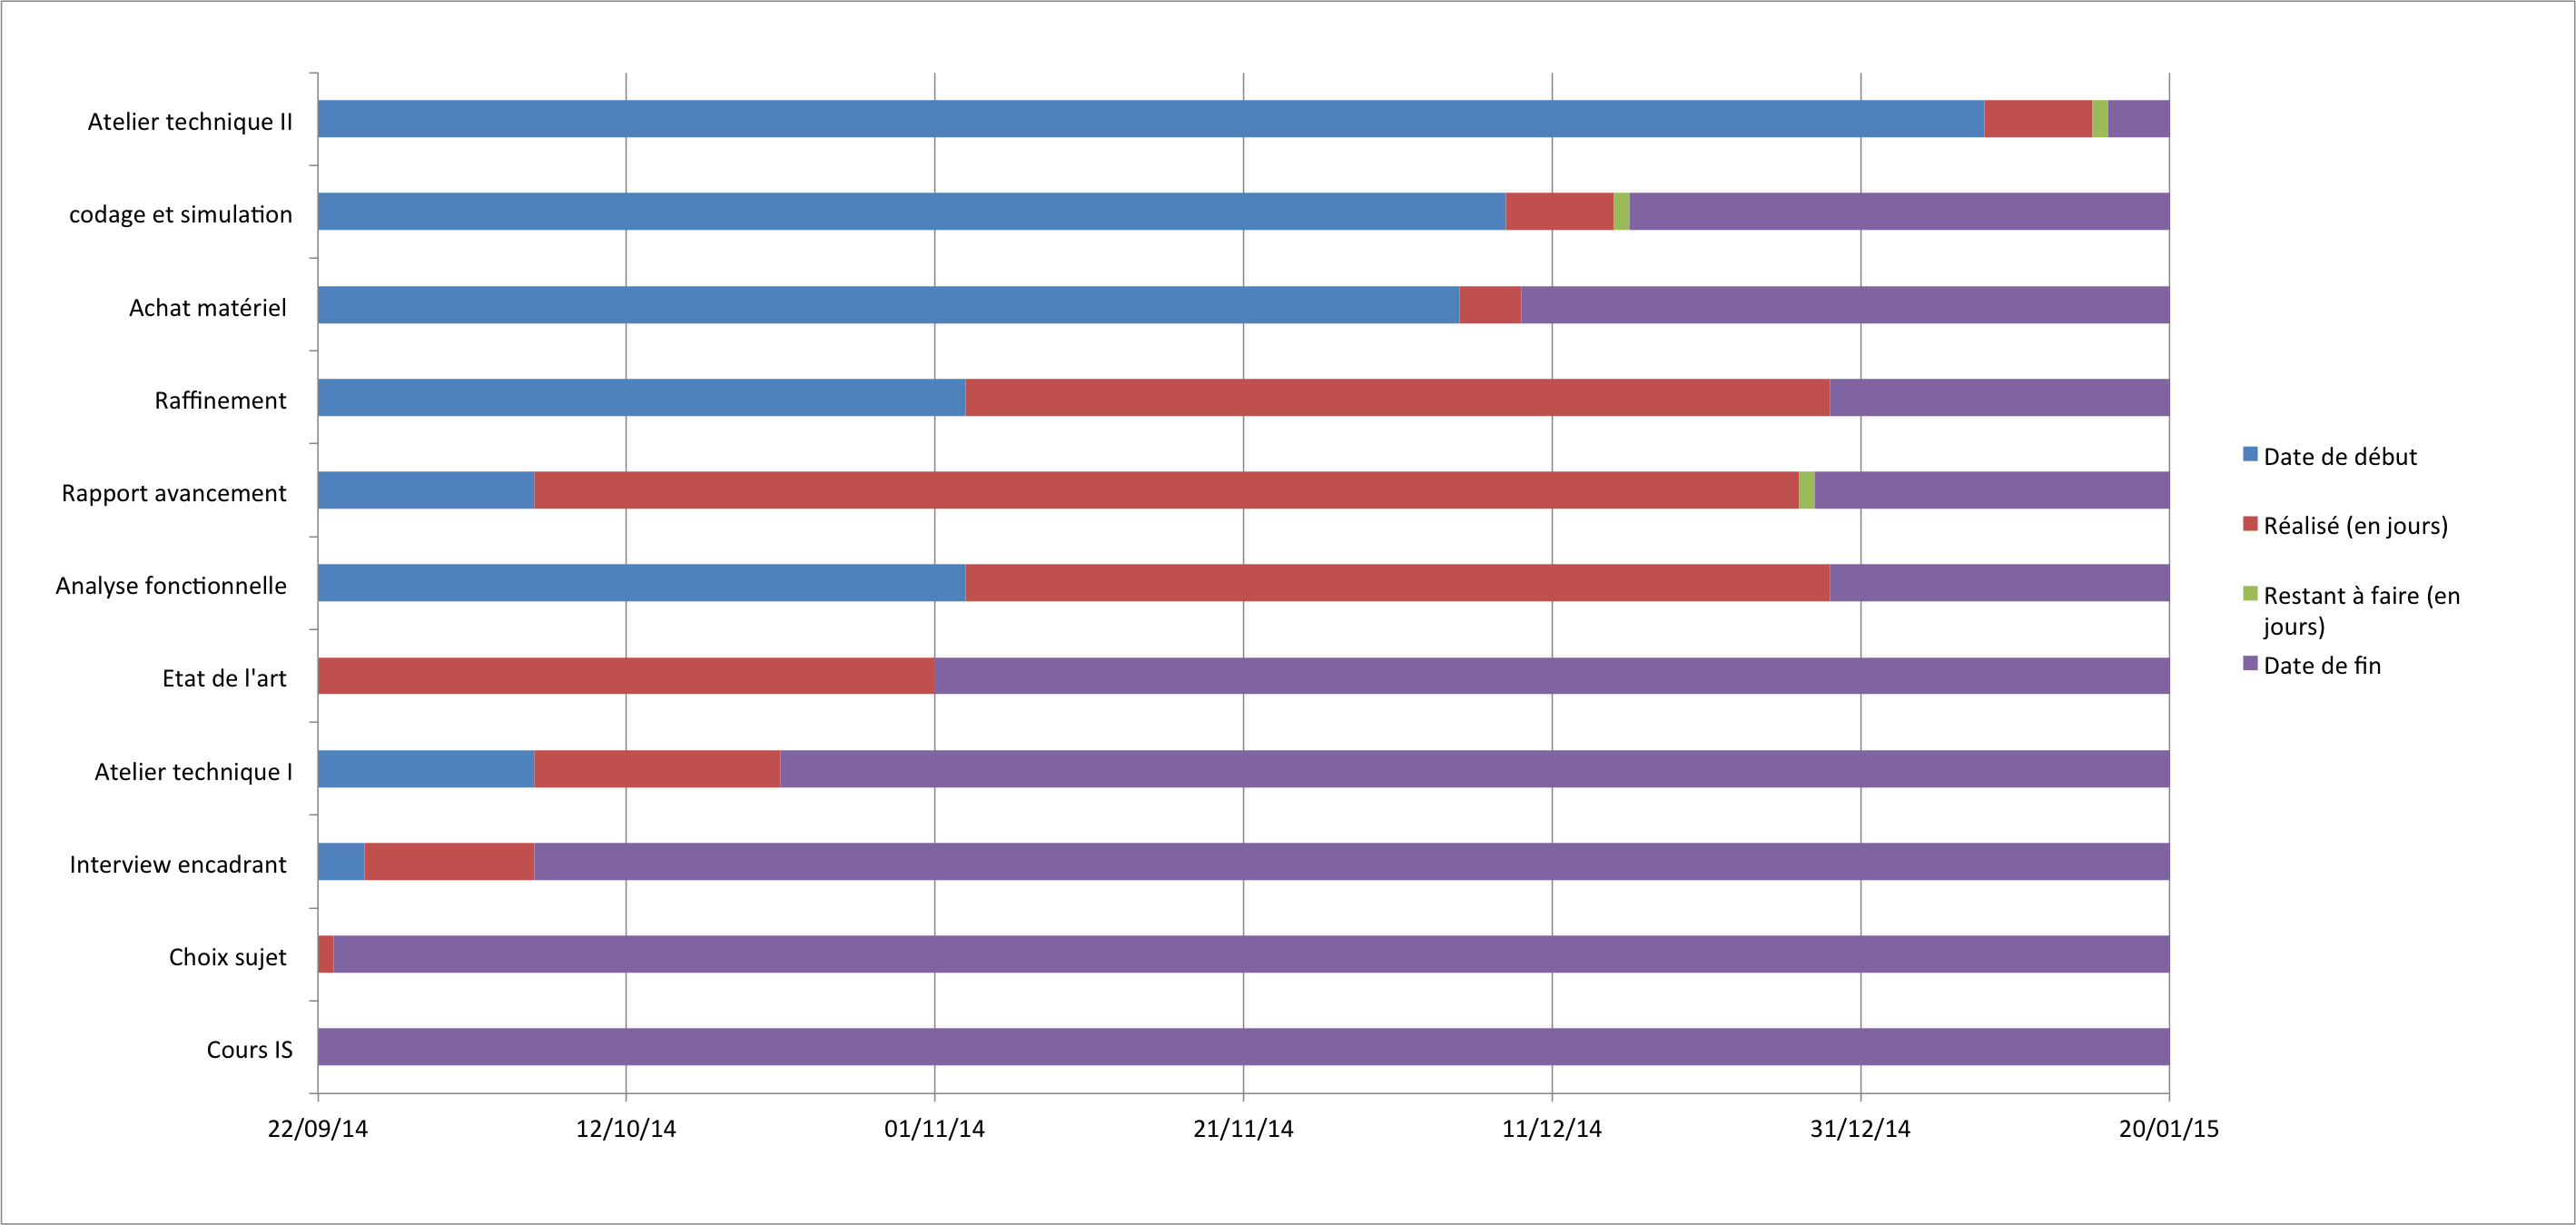
\includegraphics[scale=0.30]{GanttGraphique}
  \caption{Diagramme de Gantt version graphique semestre 1}
  \label{fig:GanttGraphique}
\end{figure}

\begin{figure}[H]
  \centering
  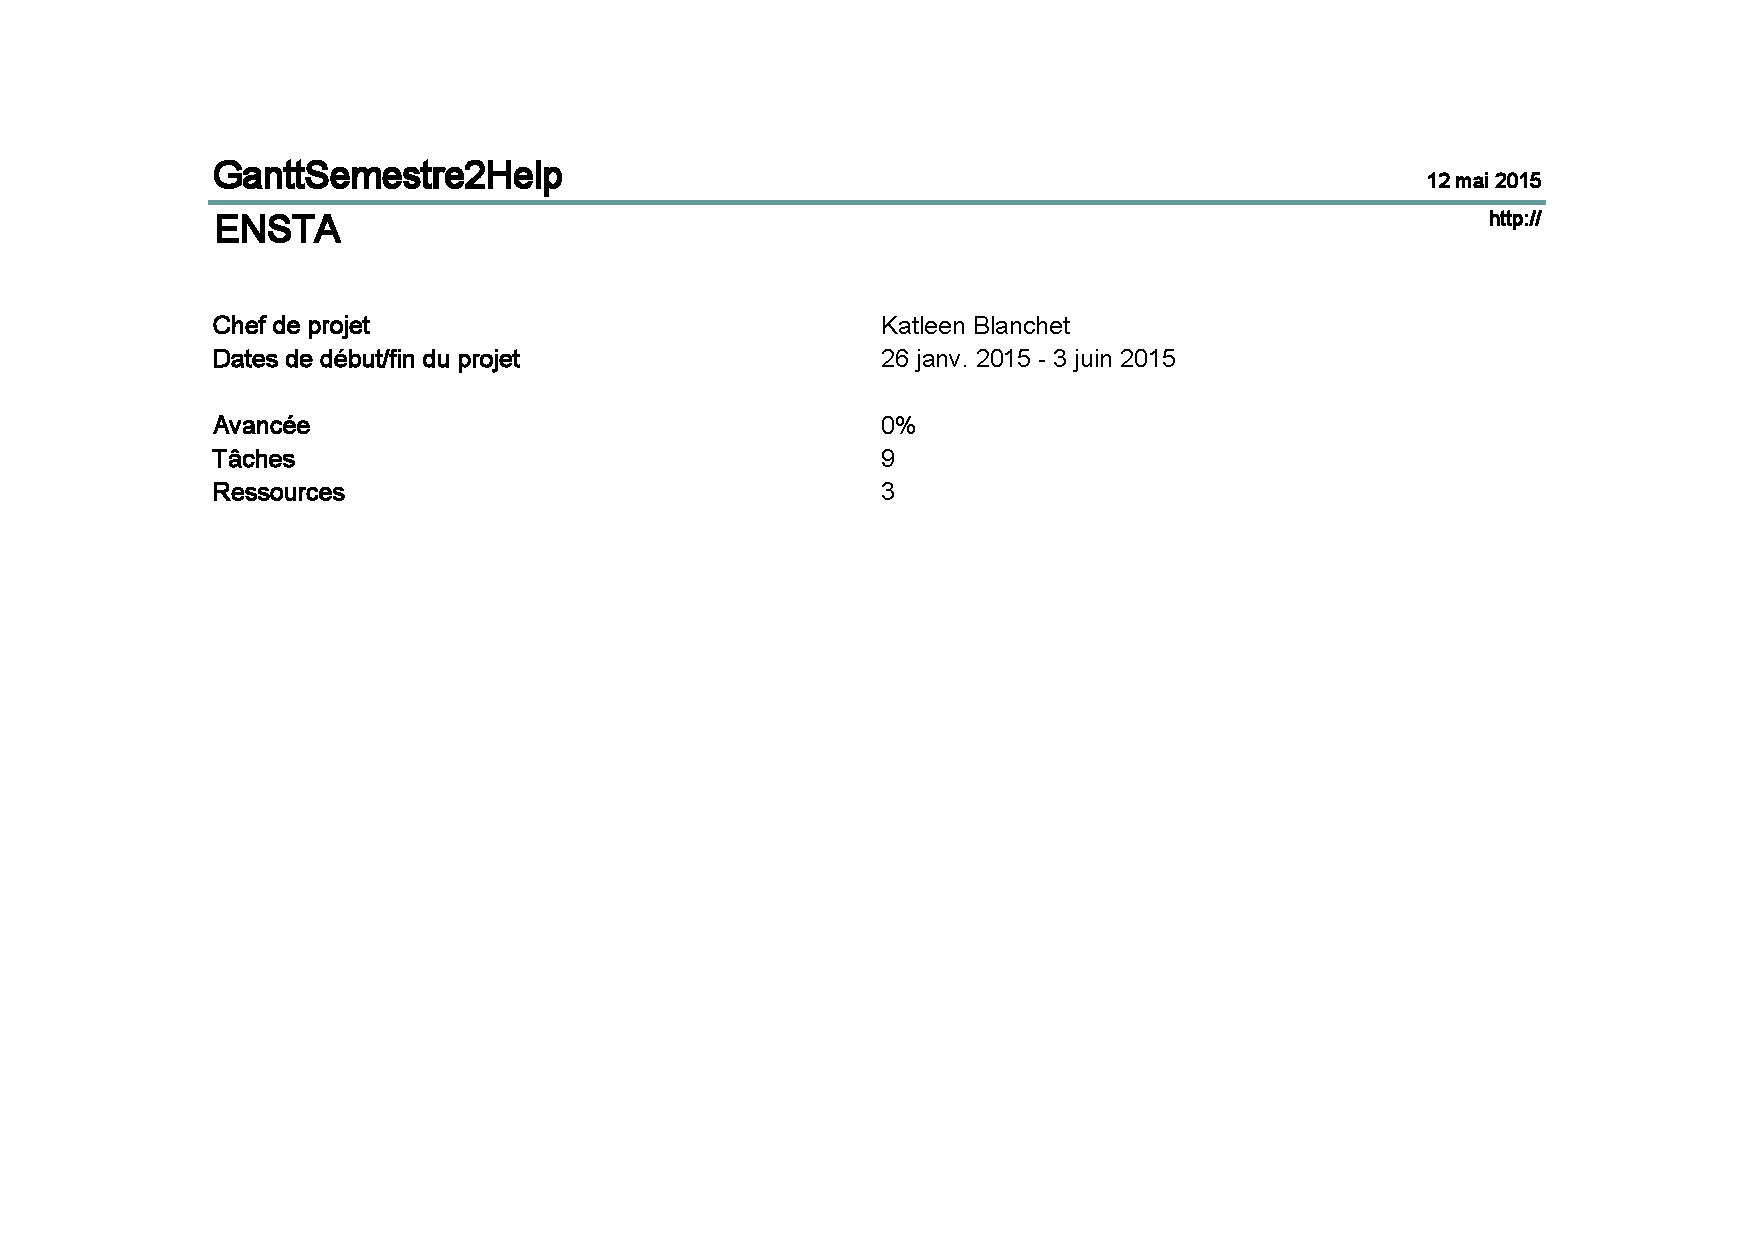
\includegraphics[scale=1]{GanttSemestre2}
  \caption{Diagramme de Gantt semestre 2}
  \label{fig:GanttSemestre2}
\end{figure}

\begin{figure}[H]
  \centering
  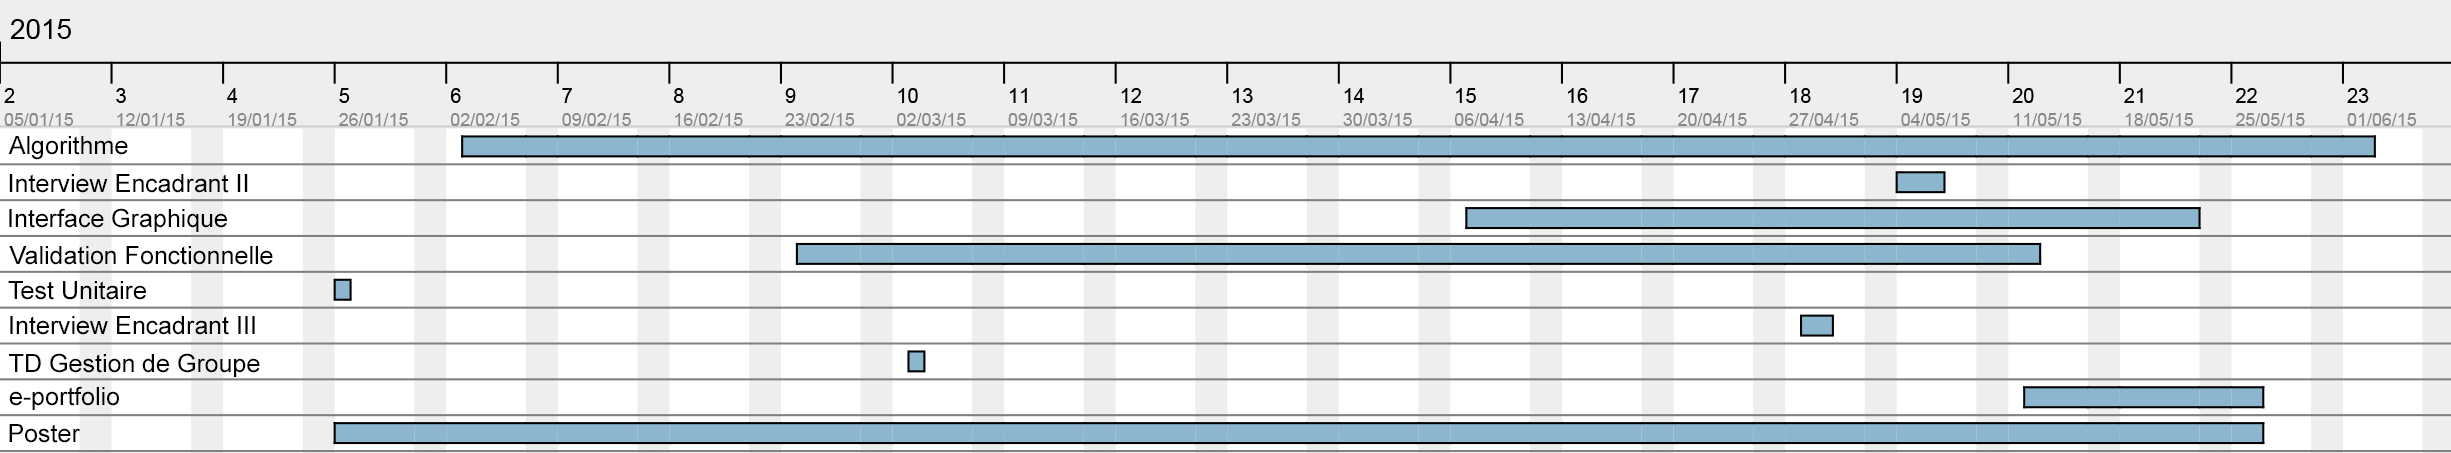
\includegraphics[scale=0.75]{GanttSemestre22}
  \caption{Diagramme de Gantt version graphique semestre 2}
  \label{fig:GanttSemestre2}
\end{figure}